

\begin{subsection}{Introducción al problema}

En este problema nos situaremos en una provincia de Optilandia, donde las ciudades están conectadas por rutas bidireccionales. Algunas de estas rutas (en general las que representan caminos más cortos y/o directos entre las ciudades) han sido catalogadas con la categoría de premium, indicando que se encuentran en mejor estado y que reciben mejor mantenimiento que el resto. Para reducir los costos del mismo existen regulaciones que impiden que una empresa de transportes utilice más de $k$ rutas premium en un mismo envío. Transportex es una de estas empresas y ha solicitado nuestros servicios para encontrar el camino de mínimo costo entre 2 ciudades (una de origen, otra de destino) cumpliendo con estas restricciones, siempre que esto sea posible.

Escribiremos un algoritmo que reciba los datos de las ciudades, las rutas y el $k$ permitido y encuentre una solución si es que existe. Las ciudades pueden interpretarse como los nodos de un grafo, y las rutas que las conectan como las aristas del mismo, por lo que interpretaremos la entrada como un grafo; también se sabe que siempre hay una forma de llegar de una ciudad a otra (independientemente del uso de rutas premium), por lo que este grafo será conexo. Llamaremos $n$ a la cantidad de nodos del grafo y $m$ al número de sus aristas. 

A partir del mismo construiremos un digrafo en el que los nodos serán de la forma $\langle c, p \rangle$, representando que se puede llegar a la ciudad $c$ utilizando a lo sumo $p$ rutas premium. As\'{i}, 2 nodos estar\'{a}n conectados sii se puede pasar de un estado a otro, formalmente,  si $c_1$ y $c_2$ est\'{a}n conectadas en el grafo de entrada, $\langle c_1, p \rangle$ y $\langle c_2, p \rangle$ estar\'{a}n conectadas si las une una ruta normal, y $\langle c_1, p \rangle$ y $\langle c_1, p + 1\rangle$ estar\'{a}n conectadas si las une una ruta premium. Tambi\'{e}n conectaremos $\langle c_1, p_1 \rangle$ y $\langle c_1, p_2 \rangle$ con $p_2 > p_1$, ya que si se ha llegado a una ciudad usando hasta cierta cantidad de rutas premium, el mismo camino sirve si la cantidad de rutas premium disponibles aumenta.

Se construye un digrafo y no un grafo ya que si $c_1$ y $c_2$ est\'{a}n conectadas por una ruta premium, tiene sentido poder avanzar desde $\langle c_1, p \rangle$ hacia $\langle c_2, p+1 \rangle$ pero no al rev\'{e}s. Este digrafo tiene $n(k+1)$ nodos ya que se genera un nodo $\langle c_1, p \rangle$ para cada $c_1 \in [0; n)$ y para cada $p \in [0; k]$; en cuanto a las aristas, cada nodo $\langle c_1, p \rangle$ tendrá $k-p$ aristas conectándolo con los nodos que representan llegar a $c1$ usando más rutas premium, obteniendose $\frac{nk(k+1)}{2}$ aristas de este tipo; a su vez tendrá a lo sumo $k$ aristas por cada arista incidente a $c_1$ en el grafo de entrada (este número cambiará en función de qué rutas sean premium y cuales no). En total, las aristas del digrafo son, a lo sumo, $\frac{nk(k+1)}{2} + mk < (n(k+1)+m)k$.

Finalmente, obtendremos el camino m\'{i}nimo entre $\langle origen, 0 \rangle$ y $\langle destino, k \rangle$, es decir, el camino m\'{i}nimo desde el origen, sin haber usado rutas premium (en realidad no se han usado rutas de ning\'{u}n tipo) y el destino, habiendo usado a lo sumo $k$ rutas premium. 
\end{subsection}


\begin{subsection}{Representaci\'{o}n}
Representamos al grafo de entrada como una matriz sim\'{e}trica $G \in \mathbb{Z}^{nxn}$, donde $G_{ij}$ contiene la distancia entre $i$ y $j$ (0 si no están conectadas o si $i=j$).  Para simplicidad, utilizamos la misma matriz para marcar si una ruta es premium o no de la siguiente manera: si $d$ es la distancia (en valor absoluto) entre 2 ciudades, $d$ será negativa si esas ciudades est\'{a}n unidas por una ruta premium, y positiva cuando las une una ruta normal. Notar que $G$ es un grafo a pesar de esta representaci\'{o}n, y que la ciudad n\'{u}mero 0 se corresponde con aquella que estaba numerada como 1 en el archivo de entrada.
El nuevo digrafo se representa por una lista de adyacencia ("lista de vecinos") donde cada vecino tiene el nodo correspondiente y la distancia. Dado que la información sobre si una ruta es premium o no está contenida en la conexión entre los nodos, las distancias se guardan positivas. Por lo tanto, un vecino es una tupla $\langle nodo, distancia \rangle$ (recordar que los nodos también son tuplas y que las distancias son ahora números naturales).
\end{subsection}

\begin{subsection}{El algoritmo}
El algoritmo que resuelve el problema consta de 3 partes: la primera es la lectura del archivo de entrada, la segunda parte construye el digrafo descr\'{i}pto anteriormente y la tercera parte ejecuta el algoritmo de Dijkstra sobre el mismo. Dado que leer un archivo y construir una matriz es trivial y que el algoritmo de dijsktra puede ser consultado de diversas fuentes, mostramos a continuación el armado del digrafo:

\begin{algorithm}[H]
  \begin{algorithmic}[1]
    \Function{Problema1-armarDigrafo}{grafoDeEntrada: int[n][n], n: unsigned, origen: nodo, destino: nodo, k}
    \State 	grafo = listaAdyacencia(n*(k+1), false)
     \For{i=0 to n*(k+1)} \Comment{Generar el digrafo que representa el problema}
		\State $c_1$ = $\lfloor i / (k+1)\rfloor$ 
        \State $p_1$ =  i \% (k+1)
        \For{j=0 to n*(k+1)}
        	\State $c_2$ = $\lfloor j / (k+1)\rfloor$ 
			\State {$p_2$ =  j \% (k+1)}
     
            \algstore{problema1}            
    \end{algorithmic}
\end{algorithm}

\begin{algorithm}[H]
	\begin{algorithmic}[1]
    	\algrestore{problema1}
        
            \If{$c_1$ == $c_2$ $\wedge$ $p_1 < p_2$}
            \State grafo.agregarVecino(i, $\langle \langle c_2,p_2 \rangle, 0\rangle)$
            \Else
            	\State distancia = grafoDeEntrada[$c_1$][$c_2$]  \Comment{distancia entre las ciudades $c_1$ y $c_2$}
                \IIf{distancia == 0} continuarConSiguienteIteracion 
                \EndIIf \Comment{Si las ciudades no est\'{a}n conectadas no hay nada que hacer}
                \State esRutaPremium = (distancia $<$ 0) 
                \If {(($p_2$== ($p_1$ + 1) $\wedge$ esRutaPremium) $\vee$ ($p_1$ == $p_2$ $\wedge$ !esRutaPremium))}
					\State grafo.agregarVecino(i, $\langle \langle c_2,p_2 \rangle, |distancia| \rangle$) \Comment{Inserci\'{o}n en O(1)}
                 \EndIf
            \EndIf
            \EndFor
      \EndFor
      \State \textbf{return} \textproc{caminoMinimoDijsktra}($\langle 0,0\rangle, \langle n-1, k \rangle, grafo, k$)
    \EndFunction    
  \end{algorithmic}
\end{algorithm}

\end{subsection}

Como solo nos interesa la distancia desde el origen hacia un nodo en particular, sería interesante poder cortar la ejecución de Dijsktra una vez que esa distancia ha sido hallada. Recordemos brevemente el algoritmo:

\begin{algorithm}
\begin{algorithmic}

\Function{AlgoDijsktra}{Grafo G, nodo origen, nodo destino}

	\State Inicializar $\Pi$ distancias y $Q$ cola de prioridades
    \While{$Q$ no está vacia}
    	\State $u \gets$ min($Q$)
        \For {each $v$ vertice vecino de $u$}
        	\State procesar $v$
        \EndFor
    \EndWhile
	\State \textbf{return} $\Pi(destino)$
\EndFunction

\end{algorithmic}
\end{algorithm}

Este algoritmo mantiene un invariante en el \textbf{while}: en el momento en el que un vértice $u$ es extraido de la cola, se sabe que se ha obtenido su distancia mínima al origen. Aprovechando esta característica, nuestra implementación de Dijsktra deja de iterar cuando la cola no tiene más elementos, o cuando el nodo de destino ha sido extraido de la cola y por tanto se tiene su distancia mínima.

\begin{subsection}{Complejidad}

La complejidad de la solución estará dada por las complejidades de sus 3 partes.:
\begin{itemize}
\item La lectura del archivo se realiza en O($m$), dado que la entrada tiene $m+4$ líneas por cada instancia del problema y que los accesos a una matriz son O(1) en C++. 
\item La generación del grafo es O($n^2k^2$) dado que consta de 2 ciclos anidados, cada uno con $n(k+1)$ iteraciones, y de operaciones en tiempo constante dentro de esos ciclos.
\item El algoritmo de Dijsktra se implementa utilizando una cola de prioridad con actualización de prioridades en O(1) e inicialización y búsqueda de mínimo en O($t$) (donde $t$ es la cantidad de elementos de la cola, la cuál se corresponde con la cantidad de nodos del digráfo generado en la etapa anterior). Llamemos $D$ al digrafo donde correrá este algoritmo, $n'$ a la cantidad de sus nodos y $m'$ a la cantidad de sus aristas. Se harán $n'$ extracciones de mínimo y $m'$ actualizaciones de prioridades, obteniendose una complejidad de O($(n')^2 + m'$). Dado que $n' = n(k+1)$ y $m' <  (n(k+1)+m)k$, Disjkstra correrá en O($n^2k^2 + m'$), donde $m' \in$ O($n^2k^2$). 
\end{itemize}

Juntandose todas las partes, el algoritmo correrá en O($n^2k^2$) (recordar que $m < n^2$ y que $m' \in $ O($n^2k^2$).

\subsection{Correctitud}
TODO!!!

\subsection{Experimentaci\'{o}n}

Para la experimentaci\'{o}n realizamos un generador de instancias aleatorias para este problema, que genera grafos de $n$ nodos, $m$ aristas (de las cuales $p$ son premium) y busca un camino m\'{i}nimo de $origen$ a $destino$ usando $k$ rutas premium ($n, m, p, origen, destino, k$ son par\'{a}metros para el generador) . El algoritmo del generador puede ser simplificado en 3 pasos:
\begin{itemize}
	\item Generar un camino de $n$ nodos de manera aleatoria
    \item Generar aristas entre nodos aleatorios (siempre y cuando no estuvieran conectados previamente ni sean el mismo nodo) hasta completar a $m$ ($m$ se establece entre $n-1$ y $\frac{n(n-1)}{2}$).
    \item Seleccionar $p$ aristas aleatoriamente y catalogarlas como rutas premium.
\end{itemize}

Para generar el camino se selecciona un nodo aleatoriamente como inicial, y se lo marca como el nodo actual. Luego, sobre los nodos que no han sido seleccionados se selecciona un nuevo nodo aleatoriamente, se lo convierte en vecino del nodo actual y se lo marca como el nuevo nodo actual. Este proceso se repite hasta que no queden nodos que no hayan sido seleccionados. Para el segundo y tercer paso simplemente se seleccionan nodos aleatorios y se los une o marca su ruta como premium si las condiciones están dadas; en ambos casos se descartan aquellos nodos seleccionados y que no cumplan las condiciones para asegurar que el algoritmo termine. En cuanto a las condiciones, se unen nodos distintos que no hayan sido unidos previamente y se marca como premium el camino entre dos nodos sii estos están unidos y su ruta no es premium.
Para la selecci\'{o}n aleatoria se utiliza la funci\'{o}n \textproc{rand} de C++.

A continuación se harán experimentaciones para medir complejidades y para analizar casos buenos y malos para esta solución (en términos de complejidad)

\subsubsection{Mediciones de complejidad}

El objetivo de esta experimetaci\'{o}n es el de comprobar que las complejidades te\'{o}ricas se cumplan en la implementaci\'{o}n. Dado que la misma depende de las variables $n$, $k$ y $m'n$, se realizarán experimentaciones para medir cada una de ellas por separado, fijando las otras 2. Recordemos que la complejidad teórica analizada es de O($n^2k^2 + m'$), con $m' \in$ O($n^2k^2$).

\paragraph{Complejidad sobre $n$}

Para este primer experimento $k$ y $m'$ serán fijadas en ?? y ?? respectivamente, mientras que $n$ aumentará de 100 hasta 500 dando saltos de a 10. Dicho de otro modo, se probarán instancias de tamaño $n = 100, 110, 120, ..., 500$, midiendo sus tiempos de ejecución. Para cada caso se harán 5 repeticiones y se tomará la mediana. Se espera que el crecimiento sea cuadrático, por lo que una vez obtenidos los resultados se calculará el coeficiente de pearson junto con las funciones $n$, $n^2$, $n^3$ y $n^4$ para medir la correlación de estas con los tiempos de corrida. Dado que todos son polinomios la correlación debería ser alta en todos los casos, pero $n^2$ debería tener la mayor correlación de acuerdo al análisis teórico. 

\hspace*{-1cm}{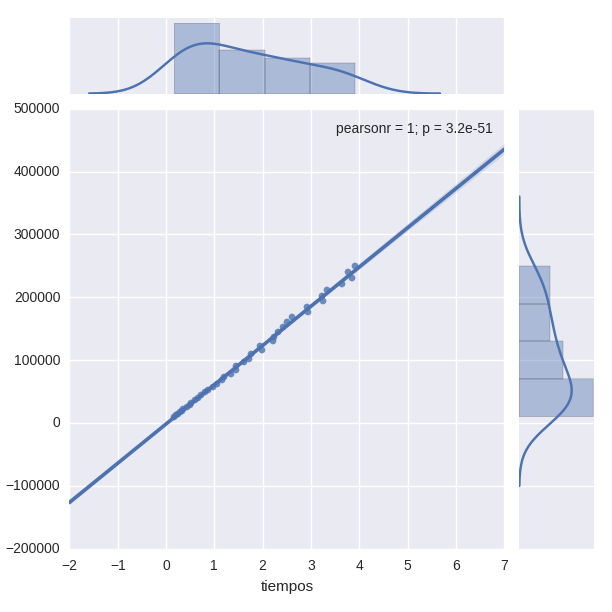
\includegraphics[width=8cm,height=8cm,keepaspectratio]{complejidad_n.png}}
\hspace*{-1cm}{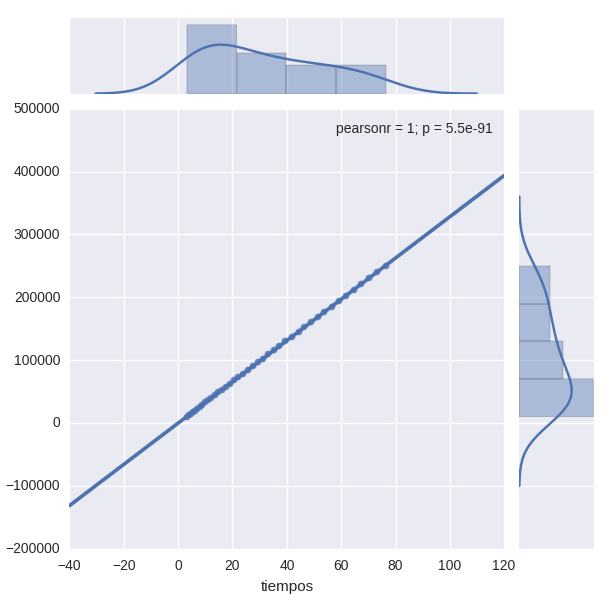
\includegraphics[width=8cm,height=8cm,keepaspectratio]{complejidad_k.png}}


\paragraph{Complejidad sobre $k$}

En este caso se fijarán $n$ y $m'$ en ?? y ?? mientras que $k$ aumentará desde 100 hasta 500 dando saltos de a 10. Nuevamente se miden tiempos de ejecución, se realizan 5 repeticiones para caso (tomando la mediana de las 5), y se mide la correlación con $n$, $n^2$, $n^3$ y $n^4$ mediante el coeficiente de pearson. También en este caso se espera que el crecimiento sea cuadrático. 



\paragraph{Complejidad sobre $m'$}

Se fijarán $n$ y $k$ en ?? y ?? y $m'$ se moverá entre 1000 y 4950 dando saltos de a 50. Nuevamente se realizarán 5 repeticiones y se tomará la mediana de los tiempos obtenidos. En cuanto al resultado esperado, recordemos que $m' \in$ O($n^2k^2$) y que $n$ y $k$ permanecen fijos, por lo que es razonable esperar que los cambios en $m'$ no aporten diferencias significativas en el tiempo de ejecución. 



\end{subsection}

